%=======================================================================
% Template para dissertação 
% Programa de Pós Graduação em Informática Aplicada da Universidade Federal 
% Rural de Pernambuco
%=======================================================================

%para incluir um arquivo por vez use \includeonly. 
%exemplos:
%\includeonly{capitulos/introducao,capitulos/bibliografia}
%\includeonly{capitulos/introducao,capitulos/conclusoes,capitulos/bibliografia}
%\includeonly{prefacios/capa2,prefacios/folha_rosto,prefacios/resumo,prefacios/abstract,capitulos/introducao,capitulos/bibliografia }

\documentclass [12pt,fleqn,oneside]{book}    % nomes e hifenação em português
\usepackage[brazil]{babel}         % Pacotes relativos à linguagem de entrada
\usepackage [utf8]{inputenc}     % aceitar texto acentuado em UTF-8
\usepackage {fancyhdr}             % cabeçalhos mais sofisticados
\usepackage {indentfirst}          % indentar 1a linha de cada seção

% Pacotes adicionados por mim
\usepackage{float}
\usepackage{nomencl}
\usepackage{multirow}
\usepackage{caption}
\usepackage{array}
\usepackage{ltablex}

% Pacotes relativos à inclusão de figuras
\usepackage {graphicx}         % para incluir figuras em PostScript
\usepackage{amsfonts,amsthm,amsopn,amssymb,latexsym}
\usepackage{geometry}
\usepackage[intlimits]{amsmath}
\usepackage{hyperref}
\usepackage{color}

% Dimensões da página
\usepackage{a4}                       % tamanho da página
\setlength{\textwidth}{16.5cm}        % largura do texto
\setlength{\textheight}{9in}        % tamanho do texto (sem head, etc)
\renewcommand{\baselinestretch}{1.4}  % espaçamento entre linhas
\addtolength{\topmargin}{-1cm}        % espaço entre o head e a margem
\setlength{\oddsidemargin}{-0.1cm}    % espaço entre o texto e a margem
\setlength{\parindent}{.0in}          % identação na 1a linha de cada parágrafo
\sloppy                               % Ser indulgente no preenchimento das linhas
\parskip 10pt                         % Espaçamento entre parágrafos

%alguns macros
\newtheorem{teo}{Teorema}[chapter]
\newtheorem{lema}[teo]{Lema}
\newtheorem{cor}[teo]{Corol\'{a}rio}
\newtheorem{prop}[teo]{Proposi\c{c}\~{a}o}
\newtheorem{defin}[teo]{Defini\c{c}\~ao}
\newtheorem{Af}[teo]{Afirma\c{c}\~{a}o}
\newtheorem{ex}[teo]{Exemplo}
\newtheorem{obs}[teo]{Observa\c{c}\~{a}o}
\newcommand{\R}{\ensuremath{\mathbb{R}}}
\newcommand{\Rn}{{\ensuremath{\mathbb{R}}}^{n}}
\newcommand{\Rm}{{\ensuremath{\mathbb{R}}}^{m}}
\newcommand{\Rnn}{{\ensuremath{\mathbb{R}}}^{ n \times n }}
\newcommand{\N}{\ensuremath{\mathbb{N}}}
\newcommand{\Z}{\ensuremath{\mathbb{Z}}}
\newcommand{\blackbox}{\rule{2mm}{2mm}}
\newcommand{\raiz}{\mbox{raiz}}
\newcommand{\contcaption}[1]{\vspace*{-0.1\baselineskip}\begin{center}#1\end{center}\vspace*{0.3\baselineskip}}

% Definindo as barras para a capa
\newcommand{\HRule}{\rule{\linewidth}{1mm}}

% Customização da Lista de Siglas
\makenomenclature
\renewcommand{\nomname}{Lista de Siglas}

% ====================================================================================


% Início do texto
\begin {document}

% Páginas sem numeração (capa, agradecimentos, etc)
\pagestyle {empty}

% Páginas iniciais
\begin{figure}[h]
\leavevmode
\begin{minipage}{\textwidth}

\includegraphics[scale=0.7]
{prefacios/capa/logo-ufrpe.eps}
\end{minipage}
\end{figure}
\vspace{-3.5cm}
{\bf
\begin{center}
{\Large
\hspace*{0cm}Universidade Federal Rural de Pernambuco \\
\hspace*{0cm}Departamento de Estatística e Informática}\\
\end{center}
}
\noindent
\begin{figure}[h]
\centering

\includegraphics[scale=0.5]{prefacios/capa/logo-bsi-presencial-v3-amp.eps}
\end{figure}


\vspace{2.5cm}
\noindent
\begin{center}
{\Large \bf Colocar o Titulo do Tcc de Thais} \\[5cm]
{\Large Thais Moura de Freitas}\\[6mm]
\end{center}


\vspace{1.5cm}
\begin{center}
{\large {\bf Recife}\\[6mm]
Janeiro de 2015}
\end{center}
\newpage
           % capa ilustrativa
%
\hyphenation{}

\vspace*{0.0cm}
{\center
{\Large Thais Moura de Freitas}\\[2.4cm]
{\huge \bf Aplicação de Uma Estratégia de Testes Automatizados Dentro do Processo de Desenvolvimento de Software}\\[2.0cm]
{\Large Orientador: Teresa Maciel}}\\[2.0cm]

{\raggedleft
\begin{minipage}[t]{8.3cm}
\setlength{\baselineskip}{0.25in}
Monografia apresentada ao Curso Bacharelado em Sistemas de Informação  da Universidade Federal Rural de Pernambuco, como requisito parcial para obtenção do título de Bacharel em Sistemas de Informação.\end{minipage}\\[2cm]}
\vspace{3cm}
{\center Recife \\[3mm]
Janeiro de 2015 \\}

\newpage
\vspace*{18cm}
{\raggedleft
\begin{minipage}[t]{6.0cm}
\setlength{\baselineskip}{0.25in}
Aos meus pais, Marcia e Abraão\\
Aos meus orientadores, Teresa e Giordano\\
Aos meus amigos\\
\end{minipage}\\[2cm]}



\newpage
\begin{center}
{\Large \bf Agradecimentos}
\end{center}
\vspace*{-0.06in}

Escrever os agradecimentos aqui nesta sessão
Escrever os agradecimentos aqui nesta sessão
Escrever os agradecimentos aqui nesta sessão
Escrever os agradecimentos aqui nesta sessão
Escrever os agradecimentos aqui nesta sessão
Escrever os agradecimentos aqui nesta sessão
Escrever os agradecimentos aqui nesta sessãoEscrever os agradecimentos aqui nesta sessão
Escrever os agradecimentos aqui nesta sessão
Escrever os agradecimentos aqui nesta sessão
Escrever os agradecimentos aqui nesta sessão
     % capa ABNT

% Numeração em romanos para páginas iniciais (sumários, listas, etc)
\pagenumbering {roman}
\pagestyle {plain}

% Geração do sumário, agradecimentos, e etc..
\chapter*{Resumo}

Escrever o resumo de thais aqui... Escrever o resumo de thais aqui... Escrever o resumo de thais aqui... Escrever o resumo de thais aqui... Escrever o resumo de thais aqui... Escrever o resumo de thais aqui... Escrever o resumo de thais aqui... Escrever o resumo de thais aqui... Escrever o resumo de thais aqui... Escrever o resumo de thais aqui... Escrever o resumo de thais aqui... Escrever o resumo de thais aqui... 

Escrever o resumo de thais aqui... Escrever o resumo de thais aqui... Escrever o resumo de thais aqui... Escrever o resumo de thais aqui... Escrever o resumo de thais aqui... Escrever o resumo de thais aqui... Escrever o resumo de thais aqui... Escrever o resumo de thais aqui... Escrever o resumo de thais aqui... 

E se quiser colocar aspas usar ``assim fica dentro das aspas``

\textbf{Palavras-chave:} Métodos ágeis, adoção ágil, lições aprendidas
         % resumo em português
\chapter*{Abstract}

Due to the necessity of high quality softwares and not enough time for activities like validation and verification, were developed software testing techniques in order to identify and correct relevant errors from the system, supporting the development and also integrating the entire application life cicle.

Amongst the techniques created, one of then is the automation of tests, that in way the running it software development if becomes a powerful strategy to minimize the effort with testing activities, especially regression testing.

In order to find as soon as possible any flaw, this work represents a test automation strategy throughout the life cycle of the development of an application. Participating in all stages of the development, carrying through activities jointly with the collaborator to cover all the possible levels of of system implementation. 

The results obtained highlight the impact of such a strategy in the accomplishment of the tests, make possible the application of tests automatized during the development and stand out the importance of the final quality of the product with this type of automation.


\textbf{Keywords:} Software testing, test automation, regression testing

\tableofcontents                    % sumário
\listoftables                       % lista de tabelas
\listoffigures                      % lista de figuras
\printnomenclature		     % lista de siglas
%\listofprograms                    % lista de programas
\clearpage


%=======================================================================
% Definir um estilo para páginas completas (cabeçalho + rodapé)
\pagestyle {fancyplain}

% Marca de capítulo do tipo "2. Blábláblá..." no cabeçalho
\renewcommand{\chaptermark}[1]{\markboth{\thechapter.\ {#1}}{}}

% Para aumentar o tamanho da caixa para o cabeçalho
\addtolength{\headheight}{\baselineskip}

% Definindo o conteúdo do cabeçalho...
\fancyhf{}
\fancyhead[L,L]{\nouppercase{\textsf{\leftmark}}} %comentar
\fancyhead[R,R]{\thepage}

% Para garantir que a primeira página de cada capítulo...
\fancypagestyle{plain}{
\fancyhf{}                          % não terá head ou foot
\renewcommand{\headrulewidth}{0pt}} % nem linhas de cabeçalho
%=======================================================================


% Capítulos são numerados em algarismos arábicos
\setcounter{page}{0} \pagenumbering{arabic}

%incluir os arquivos dos capítulos
% Os arquivos de cada capítulo devem iniciar com \chapter{Nome do Capítulo}
% (o nome deve terminar com .tex)
\chapter{Introdução}

\section{Apresentação}

No desenvolvimento de software muitos métodos ágeis, como Lean, Scrum e XP é recomendado que todas as pessoas de um projeto (programadores, gerentes, equipes de homologação e até mesmo os clientes) trabalhem controlando a qualidade do produto, todos os dias e a todo momento, pois, há evidências que prevenir defeitos é mais fácil e barato do que identificar e corrigi. Vale ressaltar ainda, que os métodos ágeis não se opõem a quaisquer revisões adicionais que sejam feitas para aumentar a qualidade \cite{inportanciaTestesAutomatizados}.

Uma importante etapa do ciclo de vida do desenvolvimento de software que compõe as metodologias ágeis é a fase que envolve os testes, pois a qualidade dos testes aplicados impacta diretamente no funcionamento estável das aplicações. Essa fase pode ser demorada e desgastante quando são executadas de forma repetitiva, principalmente se falhas forem encontradas através dos testes exploratórios ou ah-doc, o que levará o testador possivelmente a despender tempo na investigação e entendimento das reais causas do problema \cite{XiangFeng2011}.

Uma das principais razões para automatizar testes é a diminuição do tempo gasto nos testes manuais \cite{Maldonado1988}. Além de aumentar a eficiência de etapas repetitivas para reprodução de funcionalidades do sistema, especialmente em testes de regressão, onde os testes são executados iterativo e incremental após mudanças feitas no software \cite{Collins2012}.

\section{Justificativas}

A necessidade da entrega cada vez mais rápida de produtos de software faz com que o processo de teste necessite constantemente de rapidez e agilidade. Assim sendo, a automação de testes no ciclo de vida do desenvolvimento de software tem sido constantemente utilizada para suprir essa carência. É importante ressaltar que existe diferença entre testes e automação de testes, o primeiro termo se refere ao ato de testar, já automação é utilizar um software para imitar a interação do ser humano com a aplicação a ser testada \cite{Wanessa2012}.

Um fator que deve ser levado em consideração é que o tempo de execução dos testes automatizados, pois ocorre em proporções bem menores em relação ao tempo executado por um processo de teste manual, onde nem sempre o time terá tempo hábil para aplicar todos os testes planejados. Isso não exclui a possibilidade do processo de testes ser hibrido, isto é, contemplar testes manuais e automatizados. Automação de testes pode ser uma poderosa forma de testes não funcionais, por exemplo, volume, carga e regressão \cite{Bret1999}.

A automação dos testes tem como intuito a maximização da cobertura dos testes dentro do tempo disponível, para a validação e construção do software, aumentando a confiabilidade e qualidade \cite{Wissink206}. Considerando que o esforço em atividades de testes em projetos podem ser responsável por até 50\% do esforço total de desenvolvimento, automatizar o processo de testes é importante na redução e melhoria da eficácia dos testes realizados \cite{Budnik2010}. Os benefícios de tal abordagem em comparação com o teste manuais seriam: baixo custo de execução dos testes, possibilidade de replicar as sequências de teste velhas em novas versões de software (não gastando tempo com testes de regressão) e a possibilidade de realizar testes de estresse por um longo tempo de duração \cite{Wissink206}.

Ainda querendo responder a pergunta, Porque automação de testes? Segundo \cite{James2012} esses seriam os principais motivos:
\begin{itemize}
	\item Realização dos testes de regressão mais rápido para que os sistemas/aplicações possam continuar mudando ao longo do tempo, sem uma longa fase de testes no final de cada ciclo de desenvolvimento.
	\item Encontrar defeitos e problemas rapidamente, especialmente quando existe testes que podem ser executadas em máquinas de desenvolvedores, e como parte do serviço de complicação em um servidor de CI.
	\item Certificação de que pontos de integração externos estão trabalhando da forma esperada.
	\item Assegurar que o usuário pode interagir com o sistema como desejado.
	\item Auxilia no debbuging, escrita e desenho do código fonte.
	\item Ajuda a especificar o desempenho da aplicação.
\end{itemize}

No geral, com o uso de testes automatizados estamos aumentado a velocidade de entrega do projeto construído e com maior garantia de qualidade \cite{James2012}. O que ameniza o esforço gasto pelas empresas no processo com testes manuais e aumenta a cobertura de testes que não seriam realizados, por falta de tempo e esforço.

Muitas organizações costumam cair na mesma armadilha da aplicação da pirâmide de testes invertidas ou anti-padrão, como pode ser visto na imagem \cite{WatirMelon2012}.

\begin{figure}[H]
	\centering
	\captionsetup{justification=centering,margin=2cm}
	\includegraphics[scale=0.35]{capitulos/literatura/iceCreamConAntiPattern.eps}
	\caption{Pirâmide de testes anti-padrão}
	\label{fig:iceCreamConAntiPattern}
\end{figure}

Nesta figura está representado visualmente a quantidade de diferentes tipos de testes que podem ser aplicados pelo time no decorrer do desenvolvimento do software, onde é visto que boa parte dos testes são realizados manualmente e um quantidade pequena é realizada a nível unitário.

Uma parte importante  da estratégia de testes, é  saber o foco de cada tipo diferente de testes e fazer com que os diferentes tipos de testes trabalhem juntos \cite{James2012}. Por exemplo, realizar testes de unidade, com alguns testes de integração e um pequeno número de testes de aceitação. Com essa mistura é possível cobrir caminhos alternativos de testes no código, alcançar e ultrapassar barreiras de testes mais rápido aplicando os testes de unidade \cite{James2012}. A seguir é mostrada a pirâmide ideal para aplicação de teste automatizado, em que o foco não está apenas nos testes manuais e sim na base da pirâmide \cite{James2011}.

\begin{figure}[H]
	\centering
	\captionsetup{justification=centering,margin=2cm}
	\includegraphics[scale=0.35]{capitulos/literatura/automatedtestingpyramid.eps}
	\caption{Pirâmide ideal de testes}
	\label{fig:automatedtestingpyramid}
\end{figure}

Sendo assim, é de extrema importancia a aplição de tipos de estratégia de testes como esta, para o desenvolvimento de software, garantindo que o que está sendo implementado seja conforme o esperado e de forma mais rápida e automática, envolvendo todo o time na qualidade final e em todas as fases do processo. 


\section{Objetivos} 

\subsection{Objetivo Geral}

O objetivo geral deste trabalho é a implantação e cobertura de testes automatizados durante o desenvolvimento de uma aplicação que é desenvolvida com tecnologia de classificação de sinais de áudio para dar suporte a pessoas com deficiência auditiva ou surda.

\subsection{Objetivo Específicos}
Dentre os objetivos específicos deste trabalho, temos:  
\begin{itemize}
	\item Gerar conhecimento em torno de automação de testes, pesquisando e selecionando as melhores técnicas para esta proposta;
	\item Gerar conhecimento nécessário para aplicar automação dos testes da ferramenta jMIR utilizada para construção da aplicação;
	\item Investigar e selecionar as melhores técnicas e ferramentas aplicáveis na automação dos teste na aplicação escolhida;
	\item Aplicar automação de testes em todo ciclo de vida no desenvolvimento de uma aplicação;	
	\item Aplicar automação de testes para validar a integração da aplicação com a tecnologia JMIR, mais especificamente o uso do jAudio e ACE que são os componentes principais;
	\item Realizar o levantamento de quantos testes foram automatizados em cada nível da pirâmide ideal de testes durante o desenvolvimento da aplicação;
\end{itemize}


\section{Contribuições obtidas}

Com esse trabalho.... 

\section{Organização do trabalho}

Escrever a organização do trabalho...
\chapter{Referêncial Teórico}

É apresentado nesse capítulo um conjunto de definições relevantes para o tema dessa proposta de trabalho. Foi realizada uma pesquisa sistemática para selecionar os principais tópicos apoiam o entendimento deste trabalho. Os detalhes estão descritos nas próximas seções.

\section{Teste de Software}

Teste de software é o processo que realiza a avaliação do sistema ou de seus componentes com o objetivo de desvendar o comportamento para garantir que os seus requisitos estão de acordo com o esperado ou não. Em outras palavras teste é execução do sistema, a fim de identificar eventuais lacunas, erros ou requisitos que não foram implementados de acordo com as necessidades requeridas \cite{tutorialsPoint}. Segundo \cite{ansiieee1059}, Teste pode ser definido como o processo de análise do software para detectar as diferenças entre condições existentes e necessárias e avaliar as características do software.

Um bom teste pode ser aquele que tem alta probabilidade de encontrar erros que ainda não foram expostos e um teste bem sucedido é aquele que revela um erro ainda não-descoberto. O teste pode ser manual, automatizado, ou ainda a combinação de ambos \cite{Pressman2002}. A redução de custo, tempo e retrabalho são proporcionais ao quão cedo o processo de testes for iniciado \cite{tutorialsPoint}.

\section{Tipos de Teste de software}

Testes de software podem ser divididos em duas categorias, testes manuais e automatizados.

\subsection{Testes Manuais}

		Este tipo de teste é feito pela execução manual do software, ou seja, sem o uso de qualquer ferramenta automatizada ou qualquer script. O testador assume o papel do usuário final para realizar os testes e identificar qualquer comportamento que não seja esperado ou revelar defeitos. Costumam usar planos de teste, casos de teste e/ou cenários para garantir a integridade dos testes. Também pode ser incluso dentro deste tipo os testes exploratórios, no qual o testador irá explorar o software com o intuito de encontrar erros\cite{tutorialsPoint}.
		
\subsection{Testes Automatizados}

Testes automatizados podem ser definidos como automação de atividades de teste de software, incluindo o desenvolvimento e execução de scripts de testes, verificação de requisitos, como também a utilização de ferramentas de teste automatizadas \cite{Dustin1999}.
 
Entre as razões para o uso da automação dos testes de software podemos citar, por exemplo, executar testes manuais é mais demorado, uso da automação de testes aumenta a  eficiência processo, em um fatia particular temos os testes de regressão, onde os casos de testes são executados de forma iterativa, depois de alterações no software \cite{Dustin1999}.
		
\section{Níveis de testes de Software}

Em \cite{Pressman2002} aponta que a realização de testes apenas quando o sistema está construído é uma abordagem ineficaz. Segundo o autor, a estratégia de testes de software de possuir uma abordagem incremental, começando com os testes de unidades, seguindo com os testes de integração, culminando com os testes do sistema final e ainda acoplando testes que se enquadrem em testes de aceitação.

\subsection{Testes Funcionais}

Este tipo de teste é baseado nas especificações do software que será testado, a aplicação será testada através do fornecimento de entradas e em seguida, os resultados serão examinados para garantir a conformidade com os requisitos de tal funcionalidade \cite{tutorialsPoint}. Basicamente testar se os componentes e o sistema estão feitos, uma atividade ou uma função especifica do código está coerente com o esperado. Neste nível de teste perguntas como "O usuário poderá fazer isso?" ou "Esta função em particular funciona?" podem ser validadas tipicamente através de especificações de requisitos ou funcional \cite{Leung1990}. 

\subsection{Testes Unitários}

É a menor parte que pode ser testada do código que compõe o software, são de granulação fina, comportamento extremamente rápido, por exemplo, métodos de uma classe, uma classe ou classes que podem estar relacionadas. Não verificam o comportamento de unidades integradas com outros serviços ou dependências, garantem que sua função como unidade estão funcionando. Seu objetivo é isolar parte do programa e mostrar que partes individuais estão corretas em termos de requisitos e funcionalidades \cite{James2012}.  Existe um limite para cenários e dados que podem ser aplicados ao nível de testes de unidade, quando é nítido esse esgotamento é necessário o mistura com outras unidades do código e diferentes tipos de testes \cite{tutorialsPoint}.

\subsection{Testes de Integração}

Neste caso, é realizada a combinação de partes da aplicação que serão agrupadas para determinar se funcionamento desse conjunto está trabalhando corretamente \cite{tutorialsPoint}. Alguns defeitos não podem ser encontrados a nível unitário, mas são revelados através da integração com núcleos específicos \cite{Pachawan2014}.

\subsection{Teste de Sistema}

Após a realização dos testes de integração, uma vezes que todos os componentes foram integrados, os testes do sistema como um todo são agora efetuados para garantir que a aplicação atende aos padrões de qualidade desejado \cite{tutorialsPoint}. A aplicação é testada minuciosamente para validar especificações funcionais e técnicas, é construído um ambiente o mais próximo possível do ambiente de produção, para que os testes sejam executados em um ambiente que corresponda ao ambiente no qual o sistema será implantado. O teste do sistema nos retornará a validação dos requisitos de negócio e da arquitetura como todo da aplicação.

\subsection{Teste de Regressão}

Significa testar uma aplicação após o seu código fonte ter sido modificado para validar se ainda continua funcionando devidamente. Consiste em reexecutar casos de testes existentes e verificar se alterações de código não interfere em funcionalidades que estavam trabalhando corretamente, se foram inseridos novos erros ou causa problemas em erros que já foram reparados \cite{Leung1990}. Afim de identificar defeitos introduzidos por novas funcionalidades ou correção de defeitos.

\subsection{Testes de Aceitação}

Nível mais alto que trata da aplicação como uma caixa preta, sem dúvidas considerado um dos mais importantes entre os outros, este tipo de teste é feito na grande parte  pelo time de garantia da qualidade \cite{James2012}. Onde todo time verificará se o produto preenche as especificações solicitadas e satisfaz os requisitos dos clientes. O time responsável terá um conjunto de cenários previamente escritos e que serão usados no momento da validação. Durante a fase de validação outros cenários podem  surgir para aumentar a cobertura dos testes. Testes de aceitação não são apenas para identificação de erros de interfaces, mas também para encontrar divergências que poderão resultar em quebra ou erros graves do sistema \cite{tutorialsPoint}. Para a execução de desse tipo de testes é necessário definir critérios de aceitação a partir dos requisitos do software, estabelecendo como o teste será conduzido e a partir desses critérios, avaliar se o produto satisfaz aos requisitos \cite{SoftexRecife}.

\subsection{Testes Não-Funcionais}

Requisitos não funcionais são declarações que define as qualidades globais ou atributos a serem atendidos pelo sistema resultante \cite{Kirner1996}. Estes requisitos, ao contrário dos requisitos funcionais, não expressão nenhuma função a ser realizada pelo software, e sim comportamentos e restrições que este software deve satisfazer \cite{Cysneiros1997}. Os testes desses requisitos são normalmente executados com ajuda de ferramentas especializadas, com grande planejamento, avaliação arquitetural, aplicando técnicas avançadas \cite{tutorialsPoint}.

Alguns dos considerados mais importantes tipos de validação não funcionais são \cite{tutorialsPoint}:
\begin{itemize}
	\item Teste de Performance
	\item Teste de Carga
	\item Teste de Stress
	\item Teste de Segurança
	\item Teste de Usabilidade
	\item Teste de Portabilidade
\end{itemize}

\section{Automação de testes}

Ainda que a atividade seja complexa, o teste de software nem sempre é realizado de forma sistemática devido a diversos fatores dos projetos, como: tempo e recursos limitados, qualificação do time e dos envolvidos, complexidade e da rapidez da evolução dos sistemas. Sendo assim, a automação de testes uma importante medida para melhorar a eficiência dessas atividades \cite{Fantinato2004}.

Automação de testes é uso de um software para controlar a execução das atividades de teste de um sistema, a comparação dos resultados esperados com os resultados reais, a configuração das pré-condições de teste e outras funções de controle e relatório de teste \cite{Hooda2012}. Atualmente essa prática vem sendo difundida em processos ágeis, como também em Extreme Programmaing (XP), e até mesmo em organizações que ainda utilizam metodologias tradicionais como Rational Unified Process \cite{Lima2012}.

Segundo Fewster e Graham \cite{Fewster1999} afirmam que a automação de testes de software pode reduzir de maneira significativa e impactante o esforço necessário para execução dos testes. Assim como Molinari\cite{Molinari2010}, afirma que testes automatizados aumenta a produtividade e alcança em tempo menor os objetivos do teste. Apesar do grande poder que os testes automatizados apresentam, algumas empresas ainda resistem na aplicação de estratégias de automação de testes, sobretudo, por conta do esforço necessário para iniciar o processo e por demandar mudança na cultura da organização \cite{Lima2012}. Mais rápido que os testes manuais e menos suscetível a erros, máquinas possuem probabilidade de erro bem menor. Aprimorar e aplicar testes automatizados tem se tornado algo crucial nas empresas atualmente, segundo pesquisa realizada em 2008 pelo Forrester Research Inc.

A seguir serão citados e comentados algumas vantagens e dificuldades na implantação de testes automatizados.

\subsection{Vantagens da automação de testes}

De acordo com Fewster e Graham \cite{Fewster1999}, os principais benefícios da automação de testes de software são:

\begin{itemize}
	\item Torna a execução dos testes de regressão mais fácil, tendo em vista a reutilização de casos de testes automatizados de versões antigas em versões seguintes aplicando o esforço manual mínimo em testes manuais.
	\item Permite executar um maior número de testes em menor tempo, aumentando a frequência dos testes e trazendo mais confiança ao sistema;
	\item Execução de testes que seriam inviáveis manualmente falando, como a verificação de cálculos extremamente complexos ou testes de carga com um número alto de acessos;
	\item Aprimorar a utilização dos recursos, permitindo que os testadores reduzam o esforço em atividades repetitivas, conseguindo focar esforços em atividades de planejamento dos testes e na execução de cenários cuja automação é inviável;
	\item Permite aumentar a consistência dos resultados dos testes entre diferentes plataformas, já que as entradas e condições esperadas são as mesmas;
	\item Diminuição do “time to Market”, tendo em vista a redução do tempo do projeto dedicado aos testes;
	\item Aumentar a credibilidade e confiança na qualidade do sistema como um todo, um bom volume de testes automatizados bem planejados e executados com êxito podem trazer para o time um sentimento de confiança na qualidade do produto final.
\end{itemize}

Com base nessas vantagens é possível perceber o grande potencial da automação dos testes na melhoria das atividades que envolvem testes de software. Alguns desses benefícios podem ser evidenciados através da aplicação que será utilizada como caso de estudo desta proposta de trabalho.

\subsection{Desafios da automação de testes}

Em conformidade com Fewster e Graham \cite{Fewster1999} as principais barreiras e desafios na implantação da automação de testes de software em uma organização são:

\begin{itemize}
	\item Expectativas irreais: Automação de testes não é a solução de todos os
problemas e não deve ser vista como tal, deve ser encarada de forma realista;
	\item Prática de testes pobre: Caso o processo de testes adotado pela organização seja ineficaz, com testes mal planejados e documentação inconsistente, é necessário melhorar e corrigir o processo antes da implantação da automação.
	\item Manutenção dos testes: alguns softwares sofrem muitas modificações, o esforço de manutenção dos testes automatizados pode ser maior que o esforço de reexecuta-los manualmente;
	\item Problemas técnicos:  ferramentas de automação de testes também podem sofrer problemas, comprometendo a estratégia de automação. É necessário que haja um responsável  pela automação e tenha conhecimentos técnicos detalhados das ferramentas, para que o sua utilização seja efetiva.
	\item Questões organizacionais: a automação de testes precisa ser implementada na cultura da organização, com alocação de tempo para a escolha de ferramentas e formação, visando entender e selecionar as práticas que melhor se adequam a organização;
\end{itemize}

Diante dessas dificuldades, a implantação de testes automatizados é uma atividade complexa. Deve, dessa forma, ser bem analisada sobre sua necessidade e como deve ser adaptada ao processo atual da organização e time.

\subsection{Técnicas de automação de testes}

As principais técnicas de automação de automação de teste, presentes na literatura são: record and playback, scripts, data-driven e keyword-drivers. Essas técnicas serão expostas a seguir \cite{Fantinato2004}.

\begin{itemize}

	\item Record and playback 
	
Essa técnica se baseia na gravação das ações do usuário durante a interação com a interface gráfica do sistema, convertendo essas ações em scripts de testes que podem ser reproduzidos várias vezes for necessário. Para cada caso de teste é gravado um script de teste completo que inclui os dados de teste (dados de entrada e resultados esperados), o procedimento de teste (passo a passo que representa a lógica de execução) e as ações de teste sobre a aplicação.

Mesmo sendo considerada uma técnica simples e prática, sendo uma abordagem para testes executados poucas vezes, apresenta algumas desvantagens para uma grande quantidade de testes automatizados, com alto custo e dificuldade de manutenção, baixa taxa de reutilização, curto tempo de vida e alta sensibilidade a mudanças no software a ser testado e no ambiente
de teste.

	\item Programação de scripts 
	
É uma extensão da técnica record and playback que utilizando a programação e seus recursos para alterar os scripts gravados, permitindo alcançar uma maior quantidade de verificações de resultados esperados. Com o uso desta técnica é possível obter uma maior taxa de reutilização dos scripts de testes, maior tempo de vida, melhor manutenção e maior robustez dos scripts de teste. A aplicação sozinha dessa técnica produz uma grande quantidade de scripts de teste, visto que para cada caso de teste deve ser programado um script de teste, o qual também inclui os dados de teste e o procedimento \cite{Fantinato2004}.

	\item Data driven 
	
Consiste na extração, dos scripts de testes, os dados de entrada e armazená-los em arquivos separadamente, deixando com que os scripts possuam apenas a lógica de execução dos testes. Os dados de entrada são obtidos de um arquivo separado de acordo com cada caso de teste desenvolvido. Como principal vantagem, essa abordagem possui baixo esforço de manutenção ao adicionar, remover ou modificar um caso de teste \cite{Zambelich1998}.

	\item Keyword-driven 
	
Técnica orientada a palavras chave, consistem na extração da lógica dos scripts de teste, que passam a ter apenas ações específicas de teste sobre a aplicação, que serão identificadas por palavras-chave. Essas ações  podem ser comparadas a funções de um programa que são acionadas por palavras chave, durante a execução do caso de teste. Os passos executados pelo script são armazenados em um arquivo separado, na forma de um conjunto de palavras-chave e parâmetros de teste no próprio código, obtendo-os diretamente dos arquivos de procedimento de teste.
\end{itemize}

Na implementação de automação dos testes desta proposta, foram levantados as possíveis técnicas demonstradas aqui para serem aplicadas. Por ser um protótipo desktop que usa frameworks externos, praticamente todos os testes desenvolvidos foram baseados na técnica de Programação de Scripts. Para isso, foi possível incorporar outros recursos como a verificação automática de resultados com o jUnit, em casos de testes de unidade e integração, o Cucumber para alguns cenários demonstrativos aplicando BBD (Behaviour-Driven Development) e testes de aceitação. Essas ferramentas serão explicadas na próxima seção. Técnicas como Driven e Keyword Driven foram descartas para essa aplicação devido aos casos de testes desenvolvidos não possuírem uma grande quantidade de dados de entrada que justificasse a adoção dessas técnicas.

\subsection{Ferramentas utilizadas na automação dos testes}

Existe há discursão, desde o surgimento da área de testes de software, sobre a utilização de ferramentas que facilitem o trabalho dos profissionais de teste, tarefas como o planejamento de casos de testes, execução de testes, abertura de defeitos entre outros \cite{Solis2011}. Objetivando dar suporte a estratégia  de automação de testes apresentada neste trabalho, serão apresentadas a seguir as ferramentas que foram utilizadas.

\begin{itemize}

	\item  jUnit 

Framework open source (pacote de software livre) que facilita o desenvolvimento e a execução dos testes unitários em Java. O jUnit permite que os testes possam ser executados sequencialmente ou de forma modularizada, dessa forma, os sistemas podem ser testados em partes ou de uma única vez \cite{JUnit}. Em um visão geral, o jUnit tem o funcionamento com base na verificação das saídas dos métodos de uma classe, analisando se os mesmos apresentaram os resultados esperados, mostrando de forma visual o resultado da execução dos testes.
	
	\item Desenvolvimento orientado por comportamento (Behaviour Driven Development - BDD)
	
Concentrado na definição de especificações de granulação fina do comportamento direto do sistema, de forma que eles possam ser automatizado. BDD (Behaviour Driven Development) tem como principal objetivo a obtenção das especificações executáveis de um sistema \cite{Solis2011}. Os testes em BDD são escritos de forma clara e facilmente compreensível, fornecendo uma linguagem ubíqua específica que ajuda todos os envolvidos a captarem o contexto dos testes e participarem na escrita das especificações do sistema. Existem vários kits de ferramentas para o desenvolvimento e aplicação das técnicas de BDD, como JBehave \cite{JBehave}, Cucumber \cite{Cucumber} e RSpec \cite{RSpec}.

\end{itemize}

\subsection{Características do BDD utilizadas neste trabalho}

Com base em toda gama de atividades que constitui o desenvolvimento de software, incluindo obtenção de requisitos, análise, projeto, testes e implementação. Segundo a revisão da literatura \cite{Solis2011} existem seis principais características fundamentais que constituem o BDD, mas para esta proposta de automação de testes e uso do framework Cucumber, serão explicados as características que foram usadas para implantação neste trabalho.

\begin{itemize}

	\item Descrição de texto simples com estória de usuário e modelos de cenários
	
Utilizando textos simples para descrição de características,  estórias de usuários e cenários, não possuem um formato aleatório. Um modelo pré-definido é usado para especificá-los. Esse modelo é definido através de uma linguagem simples ubíqua que BDD fornece. Normalmente estórias de usuário são especificados usando o modelo a seguir \cite{bddIntroducing}:

\begin{figure}[H]
	\centering
	\captionsetup{justification=centering,margin=2cm}
	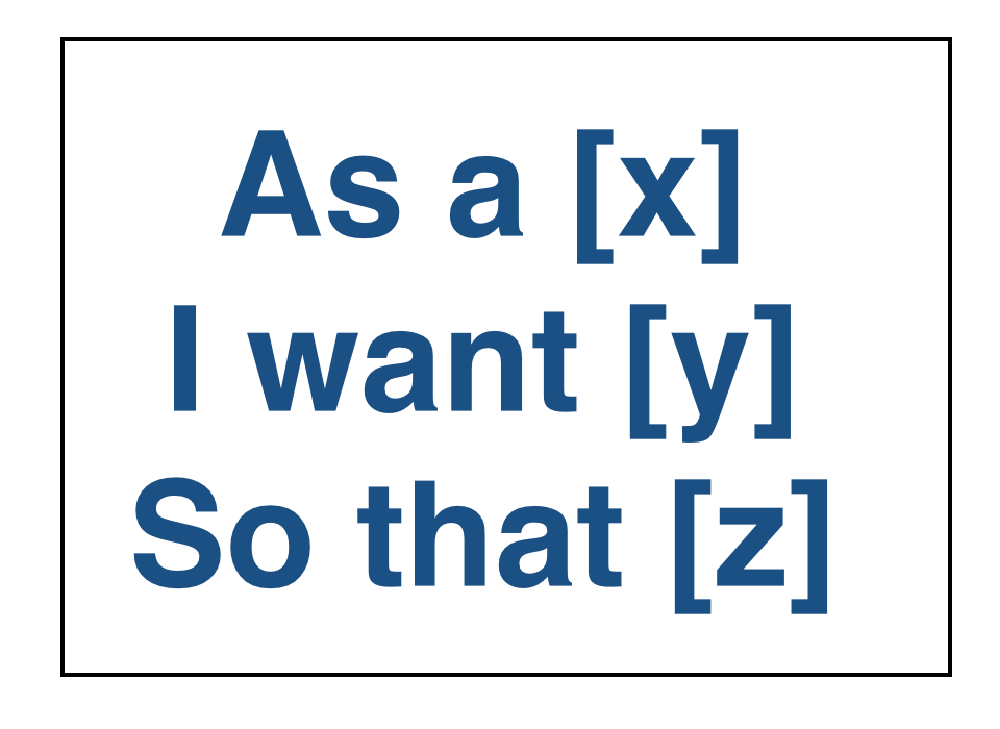
\includegraphics[scale=0.35]{capitulos/literatura/userStory.eps}
	\caption{Modelo da estrutura de uma estória do usuário}
	\label{fig:iceCreamConAntiPattern}
\end{figure}

Onde Y é o comportamento ou funcionalidade esperada, Z é o benefício ou valor desta característica e X é o papel ou pessoa beneficiada com essa funcionalidade. Para ilustrar um exemplo de como a estória do usuário pode ser escrita, temos:

\begin{figure}[H]
	\centering
	\captionsetup{justification=centering,margin=2cm}
	\includegraphics[scale=0.35]{capitulos/literatura/exemploUserStory.eps}
	\caption{Exemplo de escrita de uma estória do usuário}
	\label{fig:iceCreamConAntiPattern}
\end{figure}
	
O título da estória descreve a atividade que é realizada por um usuário em um determinado papel. A funcionalidade desejada fornecida pelo usuário, específica a característica que o sistema deve possuir , com a implementação desta funcionalidade o usuário obtém um benefício. Utilizando este modelo fica clara a necessidade de implementação de tal característica e o seu impacto para o usuário. Os desenvolvedores sabem como o sistema deve se comportar e com quem devem falar sobre tal requisito. Além disso, os usuários entram em questionamento sobre a real necessidade de tal característica, uma vez que é perguntado qual ganho ele terá com essa implementação.


Um cenário descreve a forma como o sistema  deve se comportar quando está em um estado específico e um evento acontece, para que a funcionalidade ou característica requisitada esteja funcionando de acordo com o esperado.  O resultado do cenário altera o estado do sistema ou produz uma saída para o usuário. Nós usamos o termo ação em vez de saída do sistema \cite{Solis2011} porque, uma ação representa qualquer comportamento de reação do sistema.	

\begin{figure}[H]
	\centering
	\captionsetup{justification=centering,margin=2cm}
	\includegraphics[scale=0.35]{capitulos/literatura/modeloCenario.eps}
	\caption{Exemplo de modelo da estrutura de um cenário}
	\label{fig:iceCreamConAntiPattern}
\end{figure}	
	
	\item Automação de testes de aceitação com regras de mapeamento

Testes de aceitação com BDD é uma especificação do comportamento do sistema, especificação executável que verifica as interações (conduta) dos objetos em vezes de só avaliar seus estados \cite{bddIntroducing}. Um cenário é composto de várias etapas, a etapa é uma abstração que representa um dos elementos do cenário que são: contexto, eventos e ações. Um exemplo do significado deles pode ser: em um caso particular de uma estória do usuário ou contexto C, quando um evento X acontece, a resposta do sistema deve ser Z. Cada passo desse é mapeado para um método de teste da aplicação. Para que um cenário passe (seja validado), é necessário que todas as suas etapas também passem, estas etapas são normalmente chamadas de "steps". A principal ideia no uso do BDD é o foco em prevenir falhas de comunicação, o que significa que todos no time estão se comunicando de maneira mais frequente, eficaz e com base em exemplos reais, não se baseando em abstrações ou em requisitos imperativos. 

Para a implementação da automação dos testes deste trabalho, foram escritos alguns cenários para demonstrar como pode ser utilizado na prática de desenvolvimento e testes com BDD (Behaviour Driven Development) usando a ferramenta Cucumber, que será explicado na próxima sessão.
\end{itemize}

\subsection{Cucumber}

Existem diversas ferramentas que possibilita a aplicação do BDD, mas para este trabalho vamos nos ater a uma delas, o Cucumber. Na utilização do Cucumber, as funcionalidades do sistema são escritas em arquivos de texto e em uma linguagem de domínio específico chamada Gherkin \cite{gherkin}, muito parecida com a linguagem natural, mas que contém algumas palavras chaves \cite{Cucumber}.  Para entender a estrutura básica que o Cucumber define para as estórias do usuário, a seguir são listados alguns conceitos.

\begin{itemize}

	\item Para o Cucumber, todas as  estórias do usuário referentes a uma funcionalidade do sistema estarão agrupadas em um arquivo com a extensão ".feature";
	\item No início de cada arquivo existe um resumo da funcionalidade com um formato bem simples: um título, qual o problema a ser resolvido, qual ator trabalha nesta história e qual o resultado desejado;
	\item Logo depois são definidos os cenários, que é estória propriamente dita ou critérios de aceitação que validam a estória, cada arquivo tem pelo menos um cenário;
	\item Cada história ou cenário é composto por uma descrição ou título, uma ou mais pré-condições, uma ou mais ações e uma ou mais verificações.
\end{itemize}

Essa é a estrutura básica de um arquivo ".fature" do Cucumber, esta definição pode ser genérica e gerar dúvidas, então para maior entendimento vamos especificar melhor como é essa estrutura e seu funcionamento. Os testes utilizando BDD são compostos, basicamente, por arquivos que especificam as funcionalidades ".feature" como mencionado e por arquivos de definição de passos "steps". Os arquivos com as funcionalidades são compostos por cenários, que exemplificam uma ou mais regras de negócio de como o sistema deve se comportar.

\begin{figure}[H]
	\centering
	\captionsetup{justification=centering,margin=2cm}
	\includegraphics[scale=0.35]{capitulos/literatura/exemoloCenario.eps}
	\caption{Ilustração de um cenário no arquivo .feature}
	\label{fig:iceCreamConAntiPattern}
\end{figure}	

Afim de aplicar alguns cenários na automação dos testes desenvolvidos neste trabalho, foi utilizado o Cucucmber-JVM [33] que da suporte a implementação do Cucumber na linguagem de programação Java.

\chapter{Metodologia}

Tendo em vista que o teste de software é uma das principais atividades da Engenharia 
de Software e que demanda um grande esforço em projetos de desenvolvimento, esse 
trabalho de conclusão de curso parte do seguinte problema: como implantar uma 
solução de testes automatizados em um projeto de software, de forma que a 
cobertura dos testes esteja presente em todos os níveis do sistema, durante todo o 
ciclo de vida do desenvolvimento? E quais podem ser o impacto dessa estratégia?

Para responder esta pergunta, o presente trabalho teve como foco realizar o  desenvolvimento dos testes automatizados da aplicação juntamente com o desenvolvimento do sistema.  Trabalhando na qualidade do código gerado desde da concepção da ideia e tendo conhecimento de toda a arquitetura afim de entender, selecionar e implantar a automação dos testes que foram necessários para validação durante todo o ciclo de vida do desenvolvimento.

Estão fora do escopo deste trabalho o entendimento e análise profunda do framework de classificação de áudio jMir, como também a inteligência na classificação de áudio por trás dos algoritmos que é utilizado.

Como parte desta proposta foram efetuadas várias atividades, a seguir serão apresentados os passos para execução da realização deste trabalho:

\section{Definição do Problema}

Com base em conhecimento prévio na área de testes em times ágeis,  foi observado todo o esforço e importância nas atividades envolvendo qualidade de software.  Lidando no dia-a-dia com impasses de falta de tempo para realizar testes manuais, a não cobertura de testes durante o desenvolvimento, a exclusão da qualidade do software durante o ciclo de vida e muitos outros pontos foram inputs para a motivação da pesquisa e implantação de automação dos testes durante o desenvolvimento e o impacto que isso poderia geral no resultado final do produto.

\section{Definição da Solução para aplicação da automação dos testes}

\begin{itemize}
	\item Pesquisa sobre tecnologias de áudio
	
Por motivações pessoais para o desenvolvimento de uma aplicação que envolvesse tecnologias que tratam e possibilitam a manipulação de áudio, uma pesquisa sobre áudio monitoramento foi realizada.  Com base nesta pesquisa, a proposta é automatizar testes de um sistema que utilizam um pacote de software que realiza a classificação de sinais sonoros. 

	\item Identificação da solução de um problema	
	
Ao encontrar ferramentas e apoio de tecnologias que consigam prover a classificação de sinais de áudio,  a realização de um Brainstorm foi feita para coletar ideias que serviram de base para a definição de um problema e criação de uma aplicação.


Brainstorm (ou Brainstorming) é um processo de geração de ideias que explora a capacidade criativa das pessoas,  por meio da produção em massa de ideias em um curto espaço de tempo, para posterior avaliação.  Foram escolhidos alguns temas para facilitar o encaminhamento de problemas envolvendo a classificação de áudio, tais como: saúde, educação, segurança, música, trânsito, redes sociais(comunicação). A fim de melhorar a identificação das áreas mencionadas, cada área possuía uma cor em um cartão. Cada rodada durava 3 minutos, para que os participantes gerassem ideias correspondentes a área selecionada, ao fim deste tempo, a área em destaque era trocada e repetia os mesmo passos. Depois da inserção de ideias, foram lidas todas as sugestões e melhor explicadas aos participantes. Dando inicio a próxima fase, que foi votar nas três melhores ideias geradas. Ao final da votação foi escolhido as três ideais mais votadas, o grupo então precisou pensar quais problemas cada ideia poderia resolver. 
	
	\item Concepção da aplicação/solução
	
Com base na ideia gerada através do Brainstorm mencionado, foi concebida a estória do usuário principal para a definição do escopo da aplicação.
 
\end{itemize}

\section{Referencial Teórico}

Definida a aplicação em que esta proposta seria aplicada, foi realizada a revisão da literatura com intuito de sintetizar os principais conceitos, definições e técnicas. Os assuntos que serviram de tema para este estudo teórico foram: Testes de Software, Tipos de Testes de Software, Níveis de Testes de Software e Automação de Testes.

\section{Seleção dos tipos de testes}

Com o escopo da aplicação definida, com o conhecimento necessário sobre quais tecnologias de classificação de áudio utilizar e com o embasamento teórico como base, foi possível realizar o reconhecimento de quais tipos de testes poderiam ser aplicados, quais tecnologias utilizar para cada tipo de testes selecionado. 

\section{Aplicação de testes automatizados ao longo do desenvolvimento}

Como parte da proposta deste trabalho, testes eram automatizado com base no código que era desenvolvido ao mesmo tempo, gerando validação do que era produzido, reparação de falhas e divergências da implementação. O desenvolvimento do sistema mencionado, foi feito em paralelo com o  trabalho de conclusão de curso do aluno Luan Reis.

\section{Analise do resultado dos testes automatizados}

Com base nos resultados da aplicação da automação dos testes durante o desenvolvimento do começo ao fim do sistema desenvolvido, foi possível levantar vários pontos como benefícios e reconhecer o impacto de tal estratégia de testes. Por fim, tornou-se concreto garantir que o sistema desenvolvido tinha todos os níveis de testes cobertos pela automação implementada. 

\section{Conclusão}

Nesta fase é realizada uma reflexão sobre viabilidade de implantar testes automatizados como parte do processo de desenvolvimento e de como isso pode trazer benefícios a qualidade final do produto.  Onde trabalhos futuros podem ser gerados através da aplicação e melhoria de estratégias como esta. 
\chapter{Automação de testes no desenvolvimento de uma aplicação}

\section{Contextualização da Aplicação}
Para realização da proposta deste trabalho, um ideia de protótipo foi gerada a partir de um Brainstorming, afim de criar uma aplicação para dispositivos móveis que fosse capaz de ajudar pessoas com deficiência auditiva ou surda, utilizando a tecnologia de classificação de sinais de áudio.

Segundo  o censo de 2010 do IBGE, 45.623.910 de pessoas, que equivalia a 23,9\% da população brasileira, declarou apresentar algum tipo de deficiência física. Sendo 9.722.163 de deficientes auditivos \cite{censo2010}. Um fator agravante desta realidade é a intensidade de sons que as pessoas estão submetidas ao decorrer do dia-a-dia. Alguns dos sons a seguir são exemplos que contribuem para a perda da audição: sons emitidos durante o tráfego de automóveis, obras em andamento, shows, boates e as músicas em volume exagerado nos fones de ouvido \cite{jornalDiaDia}. Segundo especialistas o limite saudável à exposição aos sons é de 80 decibéis (dB). Uma exposição diária acima desse limite pode causar danos irreversíveis para o indivíduo \cite{ruido}.

Para que este protótipo de sistema fosse desenvolvido, foi necessário alguns requisitos: 
\begin{itemize}
	\item Possuir uma base de áudios que serviriam para treinar o classificador, de forma que ele aprenda a classificar um som, se baseando em sons já existentes e conhecidos. Caso o som tenha sido gravado em um ambiente com pouquíssimo ruídos, o classificador terá maior chance de classificar corretamente o áudio, logo ter um som de qualidade pode interferir no resultado final. Caso o som não possua o mínimo de qualidade as chances da classificação ser errada são altas. 

	\item Utilização de uma ferramenta de extração e de classificação de áudio, para este trabalho a ferramenta escolhida foi o jMIR. O jMIR é uma suíte de software de código aberto implementado em Java para uso na recuperação de informação de musical (Musical Information Retrieve – Recuperação de Informação Musical). Oferecendo suporte  na manipulação de arquivos de áudio, como também para arquivos de formato simbólico. Possuindo ainda pacotes de softwares para: extração de características de áudio, aplicação de algoritmos de aprendizado de máquina, mineração de metadados e análise de metadados \cite{jmir}. 
\end{itemize}

Com base nestes recursos foi possível que o desenvolvimento ocorresse e a estruturação da automação dos testes acompanhasse simultaneamente esse processo. 

\section{Arquitetura da Aplicação}

Como componentes principais da estrutura do projeto foi utilizado o jAudio, ferramenta responsável pela extração de características do áudio. Este pacote pertencente ao jMIR, onde é utilizado para extração de recursos de arquivos de áudio. Essas características podem ser usadas na recuperação das informações da música ( Musical Information Retrieve – Recuperação de Informação Musical). Para realizar a classificação dos áudios foi usado a ferramenta também pertencente ao jMIR, ACE.

O ACE (Autonomous Classification Engine) é um pacote de software de meta aprendizado para a seleção, otimização e aplicação do algoritmo de máquina de aprendizado em música. ACE é projetado para aumentar a taxa de sucesso na classificação, facilitar a aplicação da máquina de aprendizado para todos os níveis de usuários e fornecer a experimentação dele com novos algoritmos \cite{ace}. Aplicação desenvolvida esta estruturada da seguinte forma: 

\begin{figure}[H]
	\centering
	\captionsetup{justification=centering,margin=2cm}
	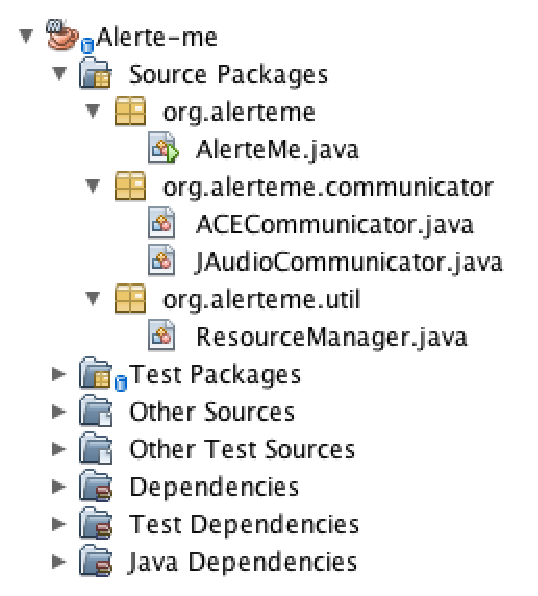
\includegraphics[scale=0.80]{capitulos/validacao/figuras/arquiteturaDoSistemaDesenvolvido.eps}
	\caption{Arquitetura utilizada no sistema desenvolvido}
	\label{fig:result-engajamento}
\end{figure}

Com base na figura podemos ver que o projeto conta com um pacote chamado Communicator, que por sua vez estão presentes as classes ACECommunicator e JAudioCommunicator, responsáveis por executarem suas respectivas ferramentas e se comunicarem com o AlertMe. A classe AlertMe é responsável por chamar todas as classes Communicator e executa-las. O projeto possui um pacote chamado Test, neste pacote estão pacotes e classes com a tarefa de automatizar todos os testes desenvolvidos no AlertMe. 

\section{Processo de automação dos testes}

O processo de automação de testes para o sistema desenvolvido foi organizado com o intuito de unir atividades de desenvolvimento e a qualidade do software gerado em tempo de desenvolvimento e não apenas como uma atividade final de validação. Para que isso fosse possível, as atividades de automação foram conduzidas juntamente com o desenvolvedor, o trabalho foi realizado iterativamente com base no que era criado para o sistema.

\begin{figure}[H]
	\centering
	\captionsetup{justification=centering,margin=2cm}
	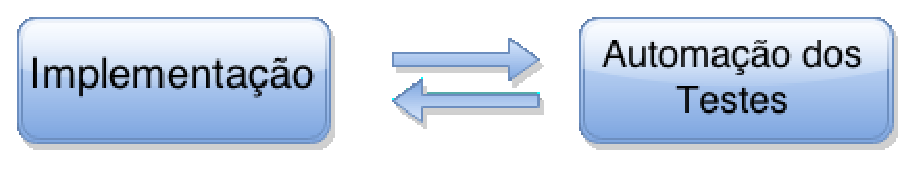
\includegraphics[scale=0.80]{capitulos/validacao/figuras/automationTestProcess.eps}
	\caption{Representação da integração do desenvolvimento e automação dos testes}
	\label{fig:result-engajamento}
\end{figure}

Foi possível observar, que a utilização dessa integração entre desenvolvimento e testes automatizados representou grande impacto na implementação e preocupação na qualidade do código produzido. Toda nova implementação realizada era validada através da automação de novos testes e a reutilização de testes que já tinham sido desenvolvidos, garantindo que essa nova versão ou funcionalidade não quebraria o sistema.

\subsection{Definição dos objetivos dos testes}

Inicialmente, foi conduzida uma análise das ferramentas que iriam compor a arquitetura do projeto: jAudio e ACE. Como elas iriam se integrar dentro da aplicação. Essa análise foi feita a partir de discussões com o desenvolvedor para entender como esses pacotes de softwares funcionavam e de como iriam ser utilizados. Essas conversas serviram muitas vezes como análise da própria arquitetura, antes da implementação e do levantamento dos testes que iriam ser automatizado. Foi possível também identificar que os testes de unidade referente ao jAudio e ACE não fariam parte do escopo deste trabalho, por serem frameworks já testados e que o principal desafio para automação proposta, seria então desenvolver testes automatizados que validassem a integração entres essas ferramentas e o sistema protótipo proposto. Logo, os objetivos da automação dos testes dessa aplicação foram a integração das ferramentas (jAudio e ACE), o funcionamento delas separadamente, mas não a nível de testar os algoritmos utilizados por ambas e sim o que era esperado como reposta da execução dessa integração.

\subsection{Implementação dos testes unitários e integração}

Depois da analise feita para identificação dos objetivos da automação e implementação do sistema, foi desenvolvida duas classes: ACECommunicator e JAudioCommunicator. Estas por sua vez, são as responsáveis por executar as ferramentas ACE e jAudio dentro da aplicação. A seguir serão listados os tipos de automação de testes desenvolvidos para cobertura de níveis unitários e de integração. As classes responsáveis por este nível de testes automatizados encontrasse dentro do pacote Communicator que pertence ao pacote de testes do projeto.  

\begin{figure}[H]
	\centering
	\captionsetup{justification=centering,margin=2cm}
	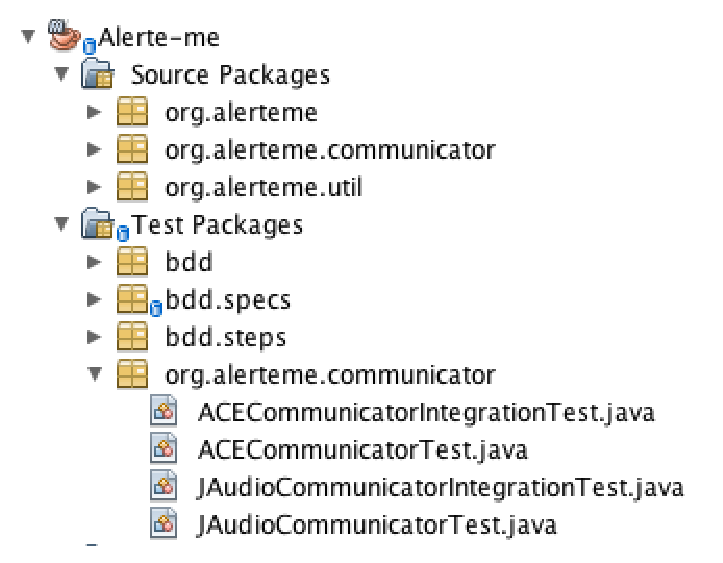
\includegraphics[scale=0.80]{capitulos/validacao/figuras/testesUnitEdIntegra.eps}
	\caption{Arquitetura dos pacotes de testes automatizados de unidade e integração, dentro do pacote de testes Communicator.}
	\label{fig:result-engajamento}
\end{figure}


\begin{itemize}
	\item jAudioCommunicator

Essa classe possui a responsabilidade de extração de características do áudio e como resposta, a criação de um arquivo “output.xml“  que irá conter todas as informações necessárias deste áudio para serem usadas na classificação.  Ela contem um método chamado extractFeatures  que recebe como parâmetro: arquivo de áudio a ser classificado, arquivo settings.xml que possui as configurações que o algoritmo de extração do jAudio necessita e nome do arquivo de output que será preenchido com as características que a extração realizará.  Para que a extração das características e o consequente uso eficaz do jAudio funcione este método precisa validar todos estes argumentos.

Nestas duas primeiras tabelas são apresentados os testes desenvolvidos para validação como unidade do jAudio e estão presentes na classe JAudioCommunicatorTeste.


\begin{figure}[H]
	\centering
	\captionsetup{justification=centering,margin=2cm}
	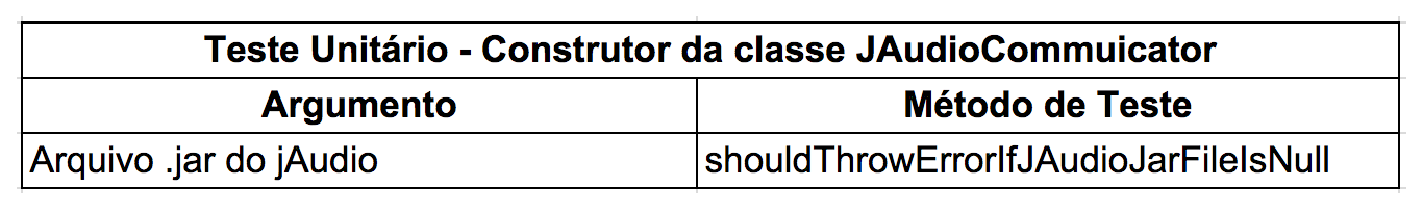
\includegraphics[scale=0.65]{capitulos/validacao/figuras/testeConstrutorJAudioCommunicator.eps}
	\caption{Teste para validação do construtor da classe JAudioCommunicator}
	\label{fig:result-engajamento}
\end{figure}
	
A validação acima garante que caso o sistema não encontre o arquivo ".jar" do jAudio, a aplicação retornará uma mensagem de erro. 

\begin{figure}[H]
	\centering
	\captionsetup{justification=centering,margin=2cm}
	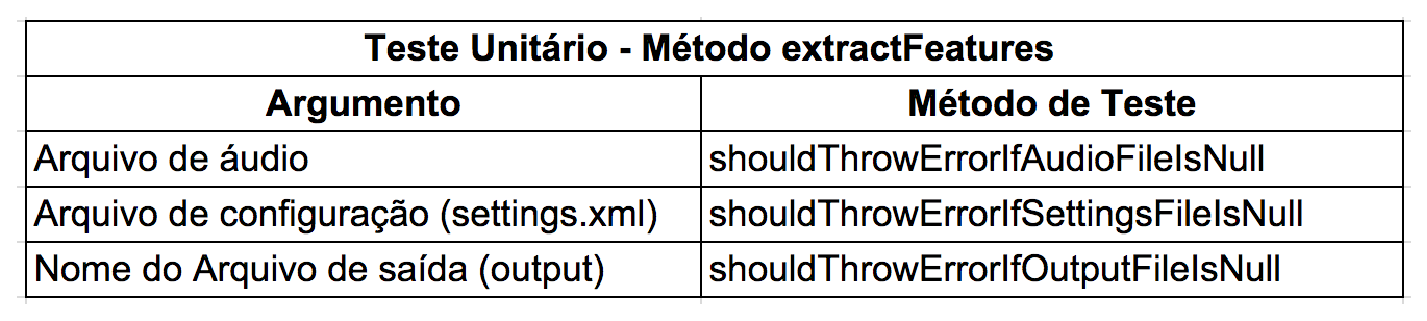
\includegraphics[scale=0.65]{capitulos/validacao/figuras/testeUniJaudioCommunicator.eps}
	\caption{Implementação dos testes unitários para classe JAudioCommunicator}
	\label{fig:result-engajamento}
\end{figure}

Esses testes validam que o arquivo de áudio, arquivo de configuração e o nome do arquivo de saída não são nulos. Todos os testes garantem que caso um destes arquivos não sejam encontrados ou estejam nulos a aplicação retornará uma mensagem facilitando a vida do usuário para entender qual o erro aconteceu e onde aconteceu. 

Como resultado da extração das características do áudio, temos a criação de dois arquivos de output, o outputFeatureVector e o outputFeatureKey. Alguns testes de integração para validação da criação destes arquivos de output foram desenvolvidos:

\begin{figure}[H]
	\centering
	\captionsetup{justification=centering,margin=2cm}
	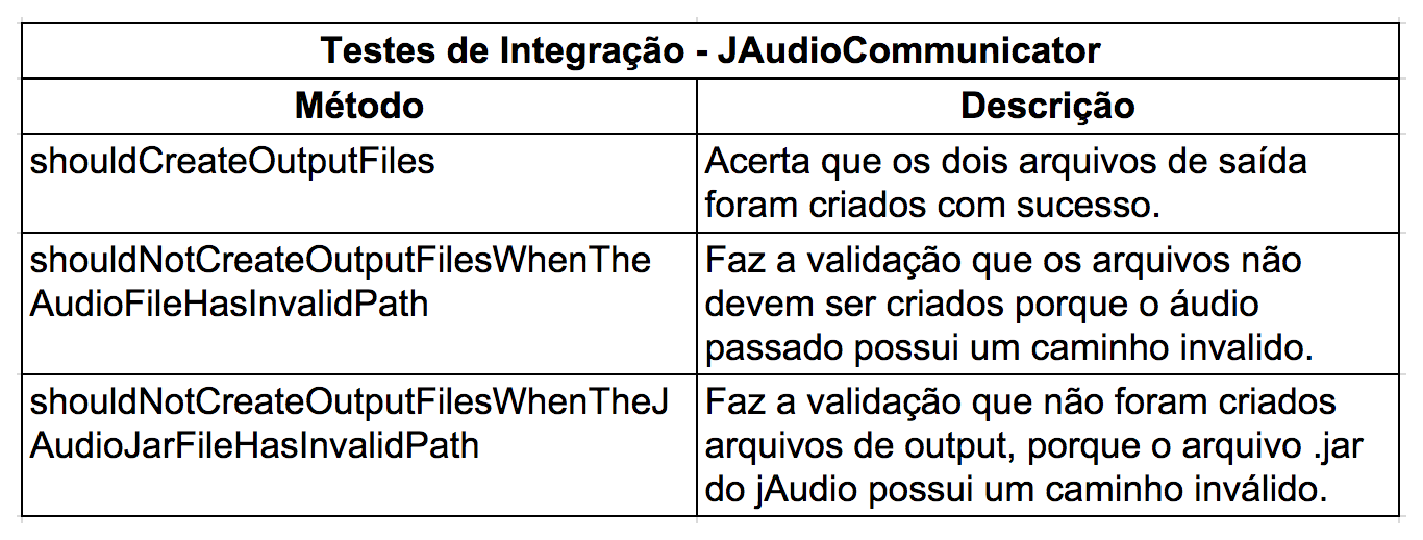
\includegraphics[scale=0.65]{capitulos/validacao/figuras/testesIntegracaoJAudioCommunicator.eps}
	\caption{Implementação dos testes de integração para classe JAudioCommunicator}
	\label{fig:result-engajamento}
\end{figure}
	
Estes testes estão em uma classe chamada JAudioCommunicatorIntegrationTest, pois necessitam de arquivos que servem como entrada para realizar o teste e validar a integração do jAudio com a aplicação. 	
	
	\item ACECommunicator

Esta classe é responsável em executar o ACE e integra-lo com o sistema, é esta classe que possui um método chamado classify, responsável na realização de fato da classificação do arquivo de áudio que foi passado para o jAudio. Para que a realização da classificação ocorra, este método recebe alguns parâmetros. Os parâmetros são: taxonomyFile, featureKeyFile, featureVectorFile, trainedMachineFile.  A figura a seguir mostra uma tabela com os métodos que cobrem a validação destes parâmetros e do arquivo .jar que é passado como argumento do construtor da classe.

\begin{figure}[H]
	\centering
	\captionsetup{justification=centering,margin=2cm}
	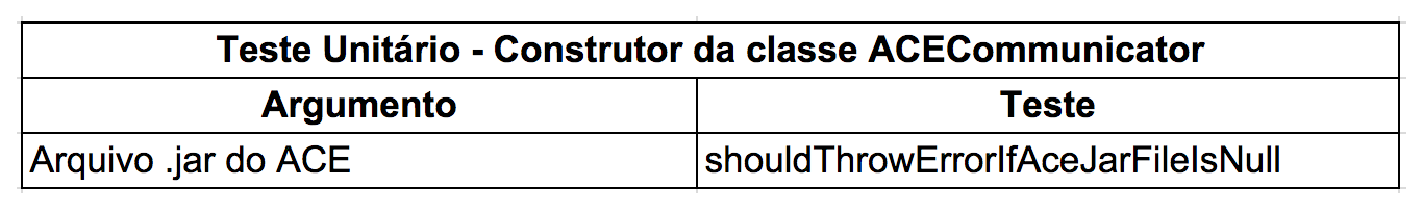
\includegraphics[scale=0.65]{capitulos/validacao/figuras/testeConstrutorACECommunicator.eps}
	\caption{Teste para validação do construtor da classe ACECommunicator}
	\label{fig:result-engajamento}
\end{figure}

Este método de teste garante que caso a classe ACECommunicator não encontre o ".jar" será lançada uma exceção para notificar que o arquivo não foi encontrado.

A seguir são apresentados os testes unitários desenvolvidos para validar o ACECommunicator:

\begin{figure}[H]
	\centering
	\captionsetup{justification=centering,margin=2cm}
	\includegraphics[scale=0.65]{capitulos/validacao/figuras/testeUniACECommunicator.eps}
	\caption{Implementação dos testes unitários para classe ACECommunicator}
	\label{fig:result-engajamento}
\end{figure}

Assim como o JAudioCommunicator, esses testes garantem que caso um  arquivos não sejam encontrados ou estejam nulos a aplicação lançará uma mensagem de erro(exceções) facilitando a vida do usuário e de todo time, no entendimento de qual erro aconteceu e onde aconteceu.

Como resultado da classificação, o ACECommunicator retornará uma lista contendo: o caminho do arquivo de áudio passado e com a resposta da classificação. Para validação desta lista foram criados vários métodos que testam a integração do ACE com a aplicação, testando cenários ,por exemplo, com entradas de arquivos válidos e inválidos. Segue a lista dos métodos de testes de integração desenvolvidos para o ACECommunicator:

\begin{figure}[H]
	\centering
	\captionsetup{justification=centering,margin=2cm}
	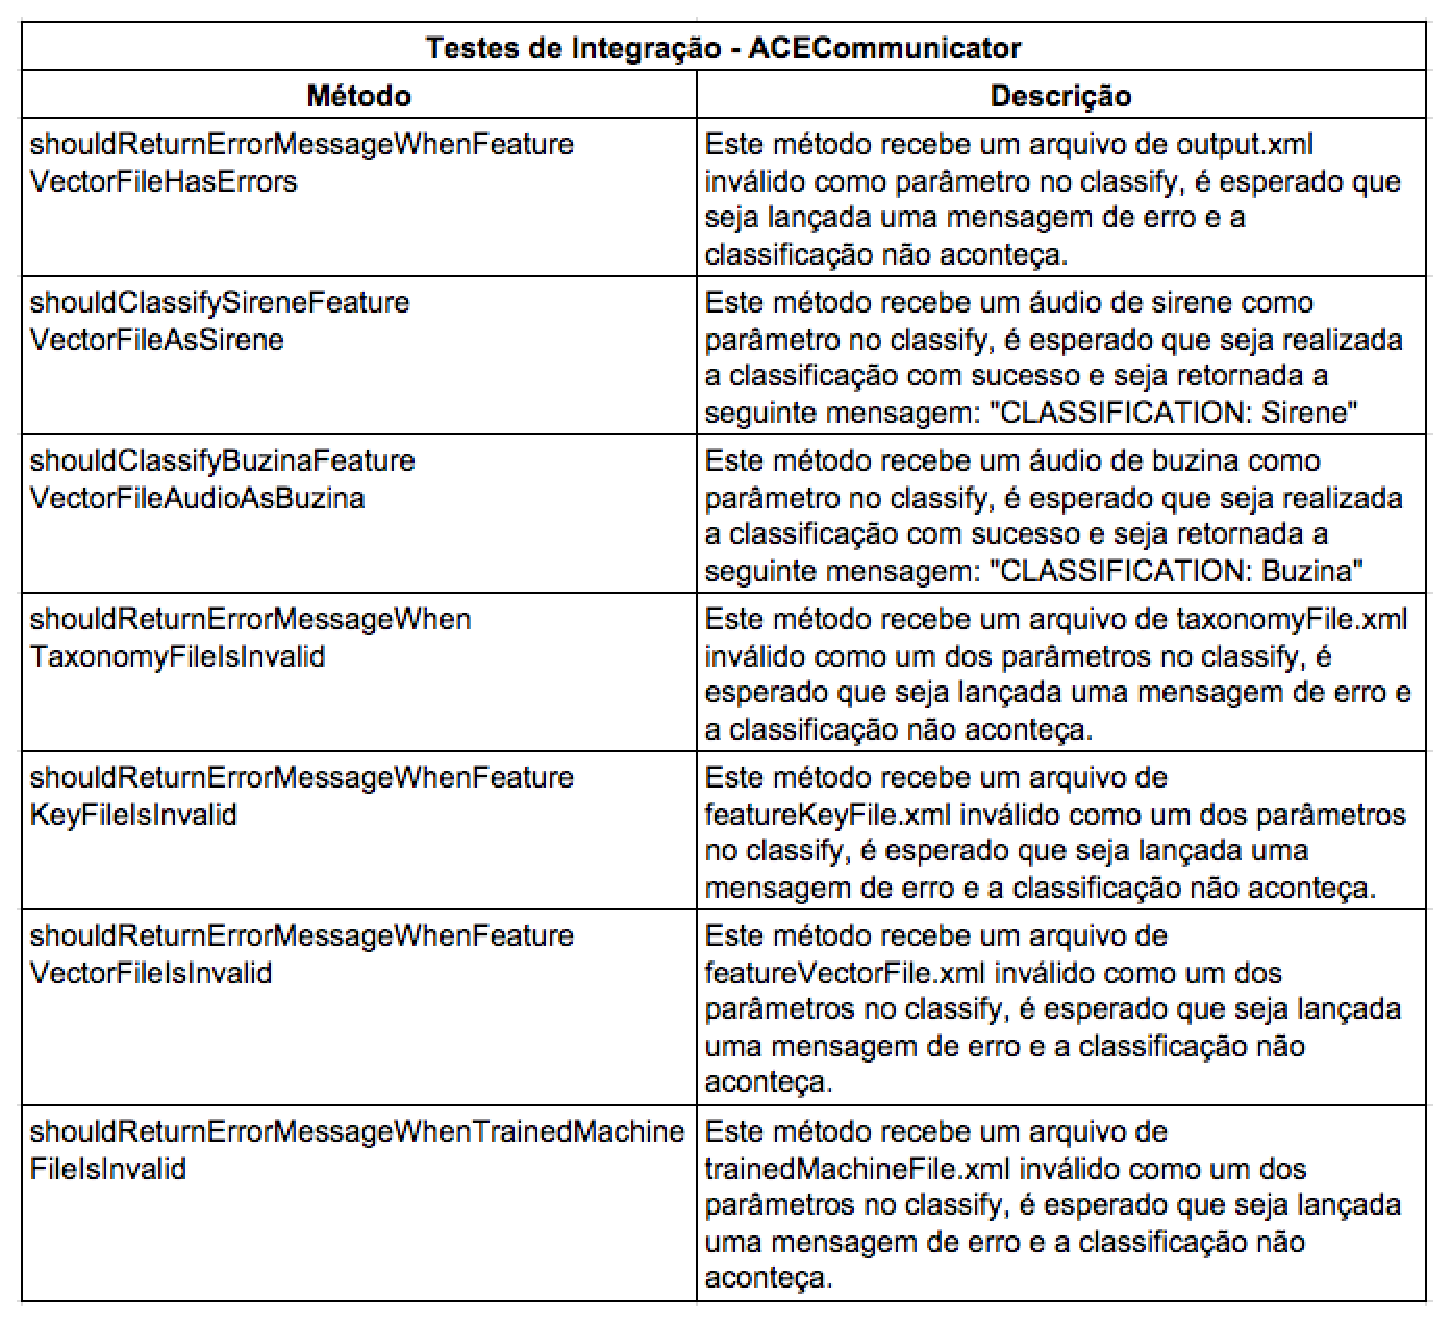
\includegraphics[scale=0.65]{capitulos/validacao/figuras/testesIntegracaoACECommunicator.eps}
	\caption{Implementação dos testes de integração para classe ACECommunicator}
	\label{fig:result-engajamento}
\end{figure}

Os testes de integração da aplicação estão em uma classe chamada ACECommunicatorIntegrationTest, dentro do mesmo pacote estão vários arquivos que foram utilizados como entradas dos cenários de testes.

Um dos métodos, responsável por testar o classify, recebeu um arquivo "invalidOutputFV.xml" (featureVectorFile) inválido como parâmetro no método classify e depois tentou realizar a classificação, mas é esperado que seja feita a validação de uma mensagem de erro para que o time ou usuário entenda porque a classificação não foi realizada com sucesso e qual foi o motivo do insucesso.

\begin{figure}[H]
	\centering
	\captionsetup{justification=centering,margin=2cm}
	\includegraphics[scale=0.55]{capitulos/validacao/figuras/exemploTesteImplementado.eps}
	\caption{Implementação de teste que valida o arquivo featureVectorFile. }
	\label{fig:result-engajamento}
\end{figure}

 Outro método implmentado, utiliza um arquivo xml vindo de um áudio de buzina válido, que foi previamente extraídas suas características com o método extractFeatures pertencente ao JAudioCommunicator, é passado como parâmetro para que o método classify realize a classificação como esperado mostrado a seguir.
 
\begin{figure}[H]
	\centering
	\captionsetup{justification=centering,margin=2cm}
	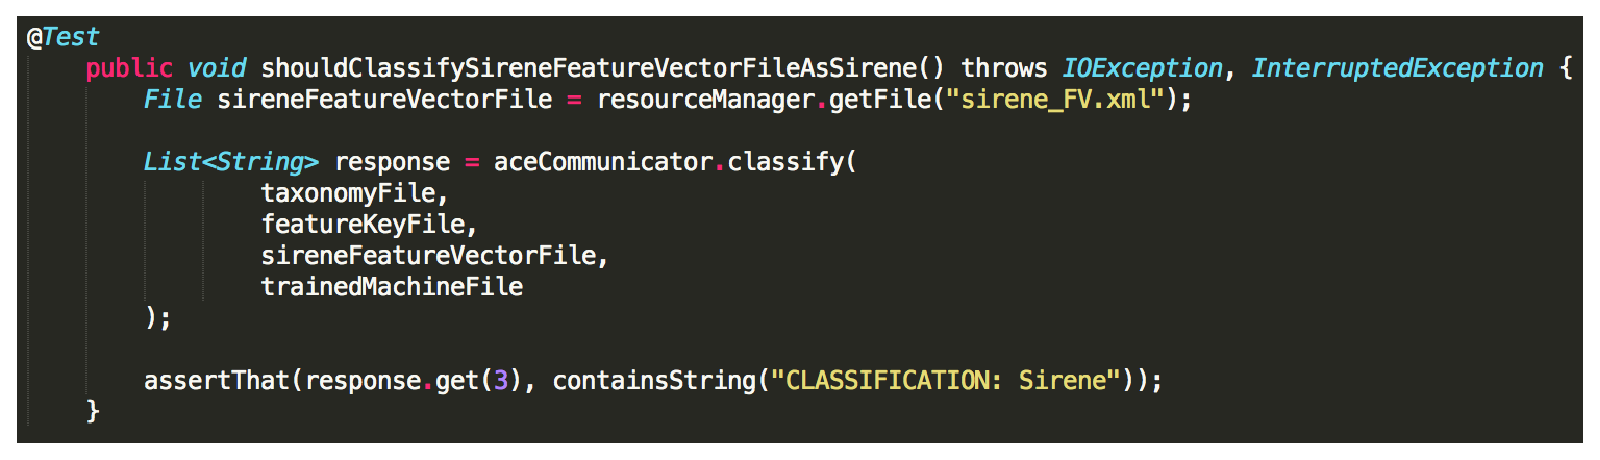
\includegraphics[scale=0.55]{capitulos/validacao/figuras/outroTesteImplementado.eps}
	\caption{Implementação de teste que valida a classificação de um áudio como sirene.}
	\label{fig:result-engajamento}
\end{figure}

\end{itemize}

\subsection{Implementando BDD com Cucumber}

O sistema inicial resultante do desenvolvimento do projeto que este trabalho automatizou os testes não possui interface ainda, mas a ideia protótipo desta interface para smartphone é que seja uma tela simples, com apenas um botão para inserir um áudio e um botão para realizar a classificação, como na ilustração a seguir:


\begin{figure}[H]
	\centering
	\captionsetup{justification=centering,margin=2cm}
	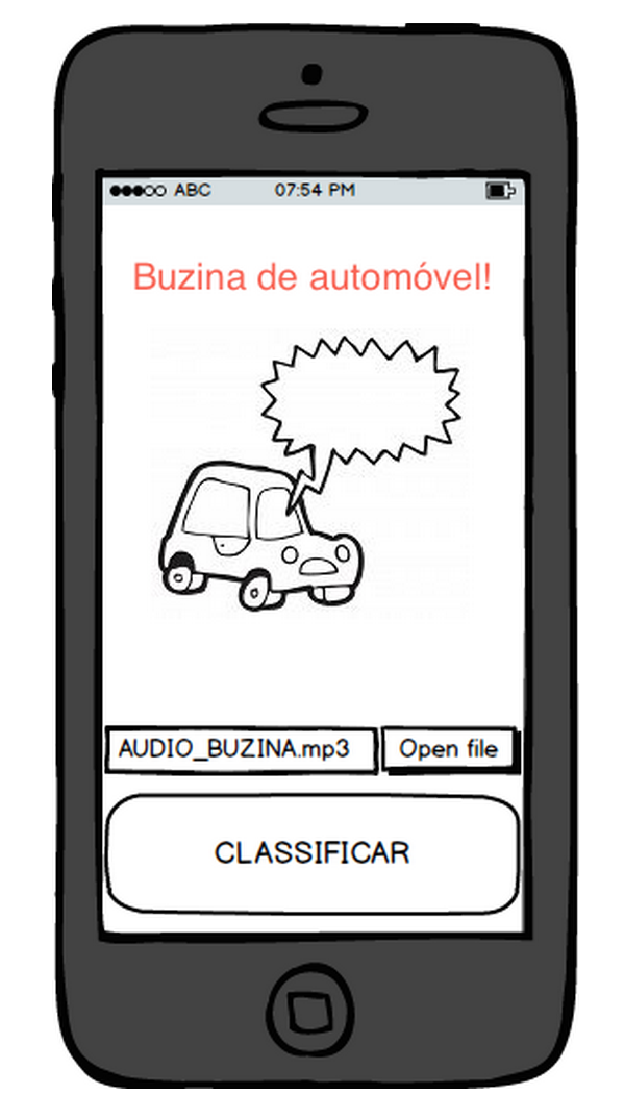
\includegraphics[scale=0.65]{capitulos/validacao/figuras/interfaceDaAplicacao.eps}
	\caption{Protótipo da interface do sistema}
	\label{fig:result-engajamento}
\end{figure}

No inicio da ideação deste projeto uma estória do usuário geral foi criada com intuito de validar a ideia gerada resultante do Brainstorm: 


\begin{figure}[H]
	\centering
	\captionsetup{justification=centering,margin=2cm}
	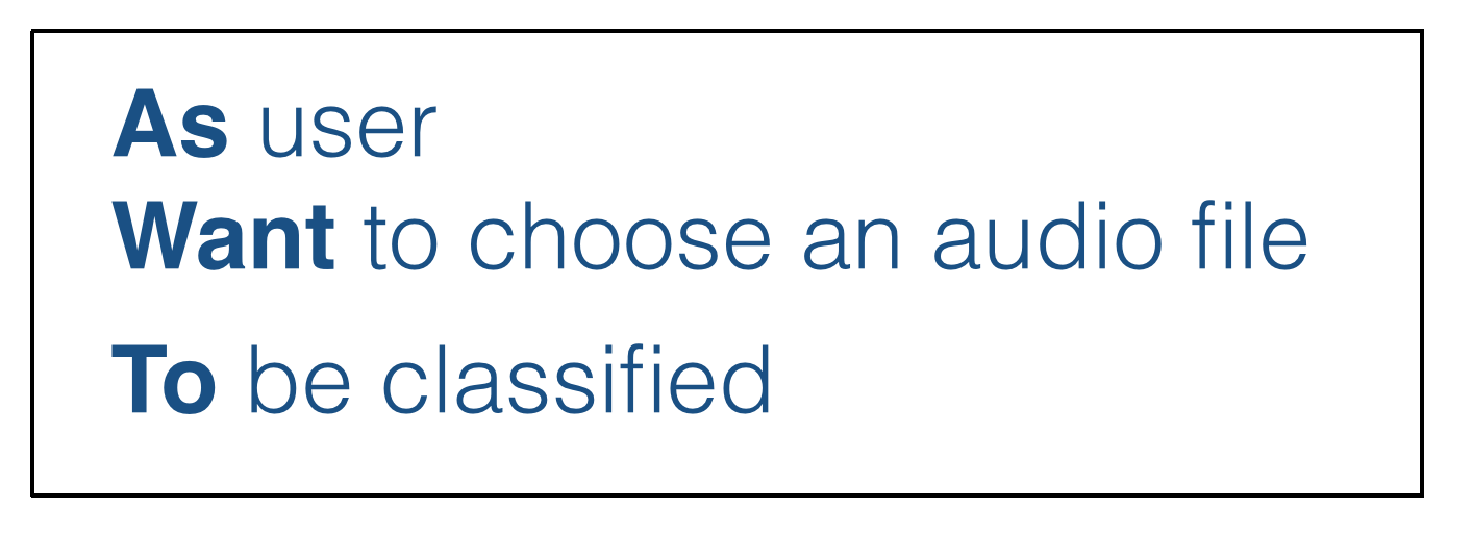
\includegraphics[scale=0.65]{capitulos/validacao/figuras/estoriaDoUsuarioDaAplicacao.eps}
	\caption{Estória do usuário desenvolvida pelo sistema}
	\label{fig:result-engajamento}
\end{figure}

Levando em consideração que o BDD nos permite a análise do comportamento que é esperado do software através da escrita de estórias do usuário com uma linguagem simples e que todos os envolvidos podem entender. Fornecendo cenários para validação do comportamento final, os cenários devem ser criados com base na estória para que validem diversos comportamentos a nível de critérios de aceitação para o cliente ou usuário. Para que a implantação dos testes utilizando BDD com Cucumber fosse possível, dentro do projeto foi criado a arquitetura que o Cucumber entende de pacotes.

\begin{figure}[H]
	\centering
	\captionsetup{justification=centering,margin=2cm}
	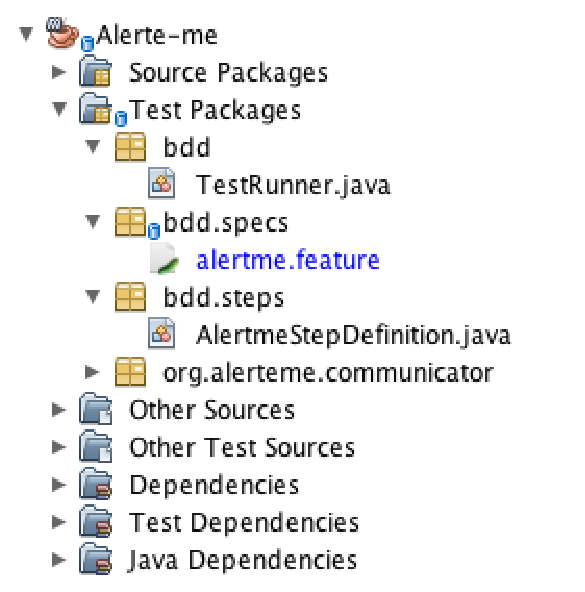
\includegraphics[scale=0.65]{capitulos/validacao/figuras/arquiteturaDeBddComCucumber.eps}
	\caption{Arquitetura dos pacotes responsáveis pela implementação dos testes de BDD com Cucumber.}
	\label{fig:result-engajamento}
\end{figure}

Dentro do pacote bdd, temos outros dois pacotes o specs e os steps. O pacote specs possui os arquivos .features e o steps possui os arquivos que implementam os passos que os cenários descrevem. Ainda na raiz do pacote BDD possuímos a classe java chamada TestRunner.java que é responsável por executar os testes Cucumber.

Foram desenvolvidos três cenários para validar a estória desta aplicação. Como teste de classificação foi usado dois áudios um de buzina e outro de sirene, que serviram para confirmar que a aplicação está realizando a classificação da forma correta. Outro cenário foi a validação de que o sistema reconhece um arquivo passado por parâmetro caso esse seja inválido.


\begin{figure}[H]
	\centering
	\captionsetup{justification=centering,margin=2cm}
	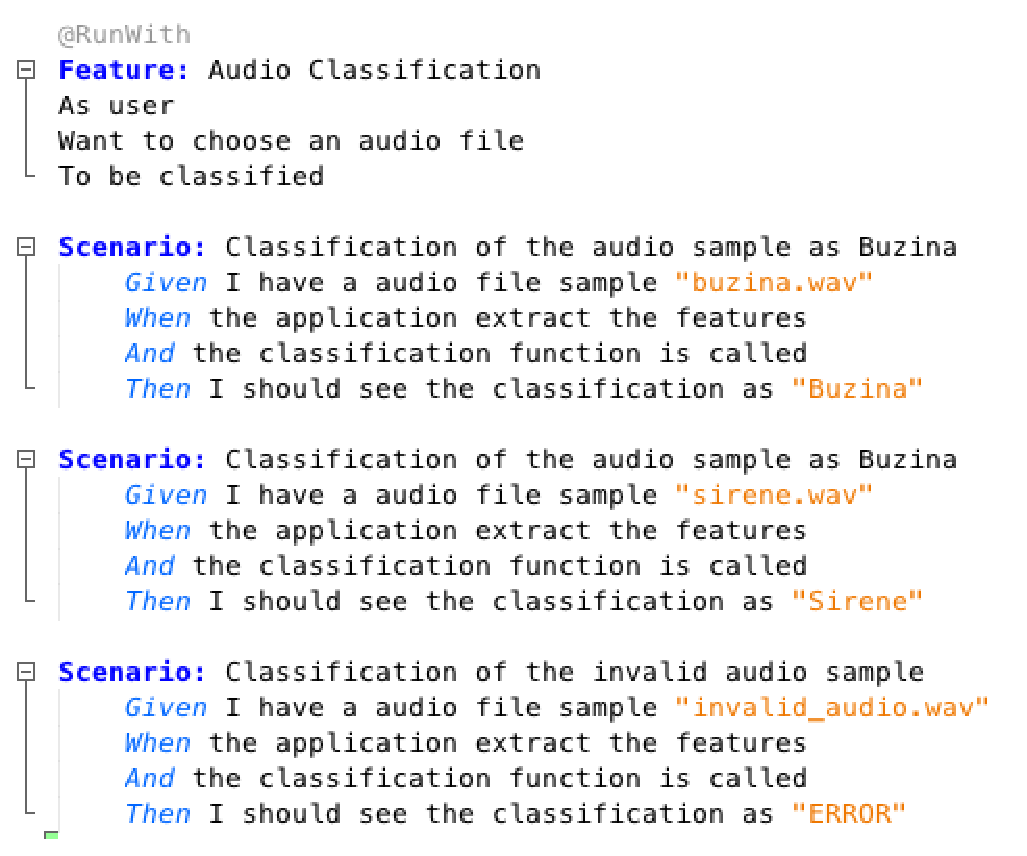
\includegraphics[scale=0.65]{capitulos/validacao/figuras/cenariosDoBDD.eps}
	\caption{Cenários de testes automatizados utilizando Cucumber}
	\label{fig:result-engajamento}
\end{figure}

Para que o Cucumber entenda estes cenários, os steps (passos) que eles possuem devem ser implementados e chamam os métodos responsáveis para que a pré-condição exista e seja validada. A seguir é possível ver a implementação de um dos cenários que foram desenvolvidos:


\begin{figure}[H]
	\centering
	\captionsetup{justification=centering,margin=2cm}
	\includegraphics[scale=0.65]{capitulos/validacao/figuras/implementacaoDeUmStep1.eps}
	\caption{Implementação dos steps de um cenário de teste com Cucumber}
	\label{fig:result-engajamento}
\end{figure}

A seguinte imagem mostra o resultado ao executarmos os cenários de testes, onde são validados e não são encontrados erros:

\begin{figure}[H]
	\centering
	\captionsetup{justification=centering,margin=2cm}
	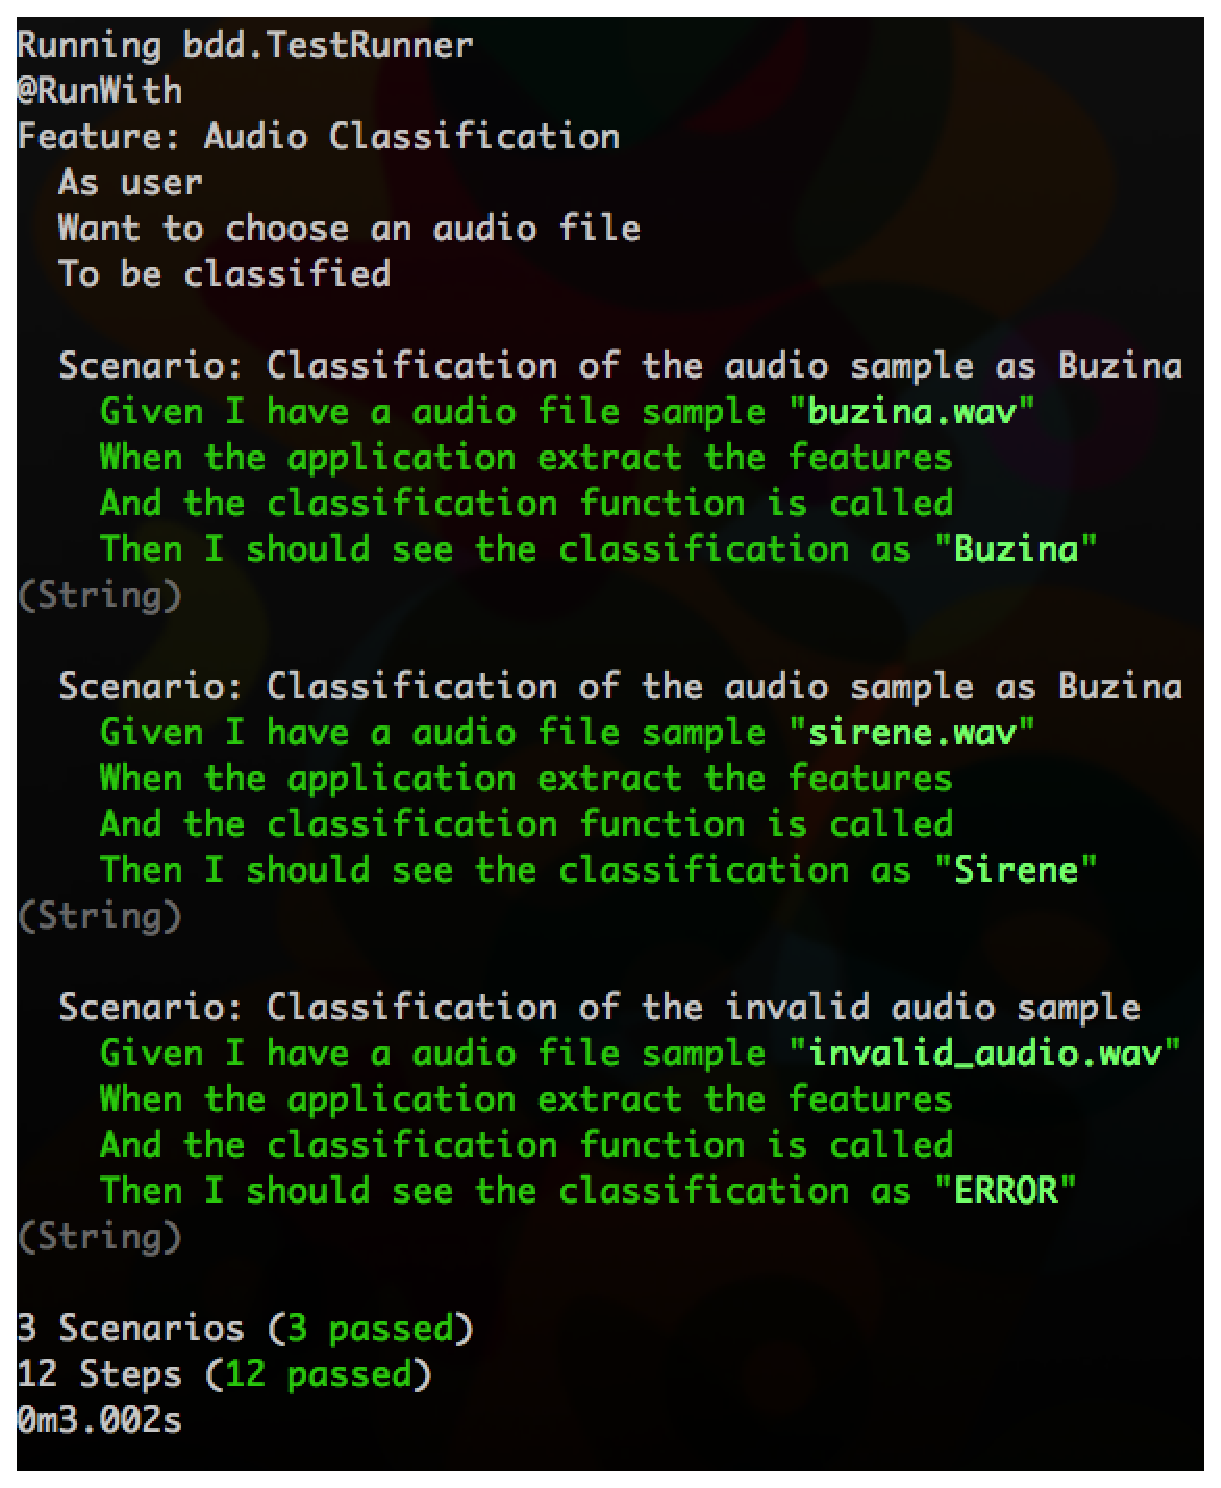
\includegraphics[scale=0.65]{capitulos/validacao/figuras/execucaoDoCucumberEtudoVerde.eps}
	\caption{Resposta da execução dos cenários de testes que foram implementados com Cucumber}
	\label{fig:result-engajamento}
\end{figure}

A figura a seguir é a demonstração de quando um dos cenários não passa ou acontece algum erro na implementação:

\begin{figure}[H]
	\centering
	\captionsetup{justification=centering,margin=2cm}
	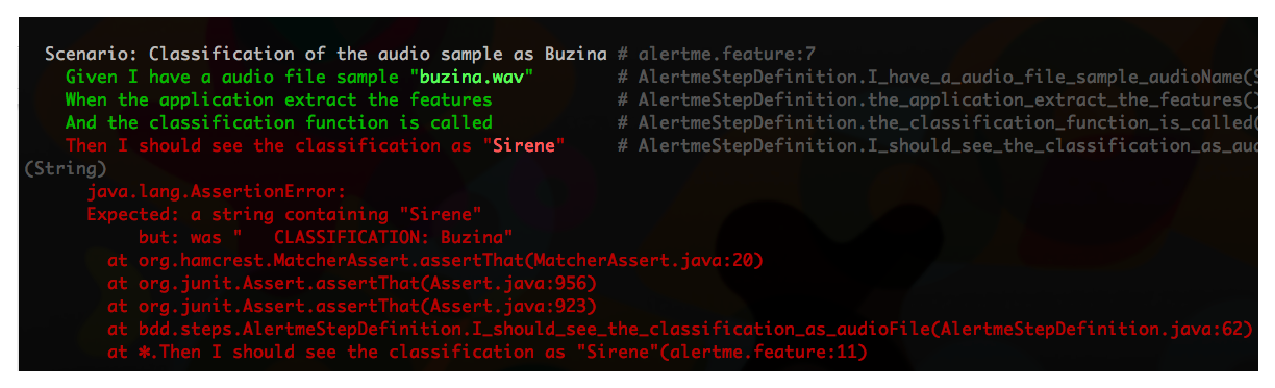
\includegraphics[scale=0.65]{capitulos/validacao/figuras/execucaoDoCucumberComUmErro.eps}
	\caption{Resposta da execução de um cenário de testes que possui um step com falha}
	\label{fig:result-engajamento}
\end{figure}

Este cenário falhou porque era esperado que o resultado da classificação fosse "Sirene" mas a classificação retornou "Buzina". Também como output da execução dos testes automatizados com Cucumber podemos ver o tempo que a execução durou, a quantidade de cenários e testes que falharam ou passaram:

\begin{figure}[H]
	\centering
	\captionsetup{justification=centering,margin=2cm}
	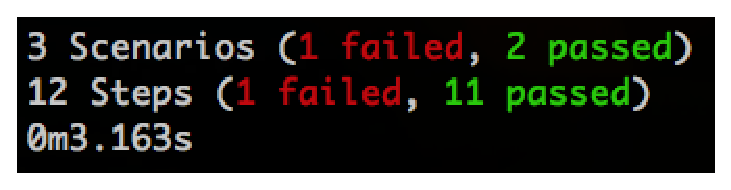
\includegraphics[scale=0.65]{capitulos/validacao/figuras/quantidadeDeErrosQpassaramOUn.eps}
	\caption{Quantidade de cenários de testes e de steps pertencentes a feature executada no Cucumber}
	\label{fig:result-engajamento}
\end{figure}

\section{Resultado da automação dos testes}
Conforme dito previamente este trabalho teve o objetivo de selecionar, implementar e analisar automação de testes durante o desenvolvimento de uma aplicação, para que todo os níveis possíveis da pirâmide de testes \cite{James2011} fossem contemplados com testes automatizados. Como observado na análise dos objetivos da automação, boa parte dos testes foram realizados para validar a integração dos pacotes de software ACE e jAudio com o sistema. O que justifica tomarmos como base para este trabalho a pirâmide a seguir: 

\begin{figure}[H]
	\centering
	\captionsetup{justification=centering,margin=2cm}
	\includegraphics[scale=0.35]{capitulos/validacao/figuras/businesstechnologyautomatedtestingpyramid.eps}
	\caption{Pirâmide de testes dividida nas faces de negócio e tecnologia.}
	\label{fig:result-engajamento}
\end{figure}

Levando em consideração a analise dos objetivos da automação, é visto que esta é a estratégia para aplicação dos testes que melhor se aplica aos resultados que foram coletados ao final deste trabalho.

Para validação da pergunta no topo da pirâmide: "Are we building the right system?" (estamos construindo o sistema certo?), foi realizada a validação com base nos testes de aceitação utilizando BDD com a ferramenta Cucumber,  onde foram desenvolvidos 3 cenários e 12 steps (passos). Este tipo de validação nos ajuda a encontrar divergências entre os principais objetivos do sistema e o seu resultado final esperado, garantindo a verificação do comportamento da aplicação. 

Conforme apresentado na figura, todos os testes de unidade e de integração se encontram na base da pirâmide, respondendo a pergunta: "Are we building the system right?" (Estamos construindo o sistema de forma correta?).  A  aplicação dos testes automatizados, realizados neste trabalho, resultou  em um total de 37 testes, onde 34 destes foram de integração mais unidade e 3 cenários(12 steps) de testes que validam aceitação. É relevante ressaltar que as ferramentas utilizadas ACE e jAudio já possuem uma gama de testes que não fazem parte do escopo desta proposta, mas que ressaltam a importância dos testes que foram realizados serem de integração. Com isso é factível assumir que o desenvolvimento foi coberto por atividades de testes automatizados desde a sua concepção até o final do desenvolvimento. Com praticamente todas as classes e integrações testadas automaticamente ao realizar alguma mudança no projeto e ao gerar um novo build. 

A imagem a seguir mostra a representação da pirâmide resultante deste projeto. 

\begin{figure}[H]
	\centering
	\captionsetup{justification=centering,margin=2cm}
	\includegraphics[scale=0.35]{capitulos/validacao/figuras/pyramid.eps}
	\caption{Pirâmide com as quantidades de testes desenvolvidos neste trabalho}
	\label{fig:result-engajamento}
\end{figure}


\chapter{Conclusão}



\section{Conclusão do Trablho}

Este trabalho teve como objetivo a implantação e cobertura de testes automatizados durante o desenvolvimento de uma aplicação que foi desenvolvida com tecnologia de classificação de sinais de áudio para dar suporte a pessoas com deficiência auditiva ou surda.

Foi possível observar que a implementação da automação dos testes desde do começo do desenvolvimento e em conjunto com o desenvolvedor (time) pode impactar no desenho da arquitetura e na melhor aplicação das ferramentas e estruturação do projeto. Ainda em tempo de desenvolvimento das funcionalidades era possível corrigir os erros que eram revelados durante a aplicação da automação dos testes.

Sendo assim, aplicação de testes automatizados em todos os níveis de testes, como a pirâmide ideal de testes indica, foi empregado através de técnicas e ferramentas que deram o suporte necessário desta implementação. Um dos benefícios percebidos foram os ganhos de tempo na execução dos testes automatizados e a frequência com eles podem ser executados, uma vezes que eles foram desenvolvidos, podem ser reproduzidos em vários ambientes e ao longo de alterações para validar novas versões a um baixo custo. Tal característica ressalta o potencial dos testes automatizados para testes de regressão.

Por fim,  é perceptível que a implantação de testes automatizados não é um processo fácil, que demanda uma mudança, tanto de como o processo de testes são executados quanto na capacitação  técnica dos responsáveis pela automatização dos testes do time, mas que sua utilização sistemática pode ser eficaz e trazer benefícios reais a um projeto de desenvolvimento de software. 


\section{Trabalhos futuros}

Em conjunto com o desenvolvimento do trabalho de conclusão de curso que foi realizado em paralelo com este, chegou se a conclusão que é factível dar continuidade ao desenvolvimento e aprimoramento da aplicação juntamente com a automação dos testes. Realizando melhorias nos próximos passos do desenvolvimento e aprimorando as técnicas e aderindo novas tecnologias para validar o quanto antes a aplicação. Ainda também garantir testes a nível final com o usuário e de interface, coletando novos dados para continuar aprofundando estudos deste tipo de estratégia.


%Incluindo referências bibliográficas
\bibliographystyle{plain} %define o estilo
\bibliography{./bibliografia/referencias} %busca o arquivo referencias.bib

% Incluindo anexos numerados com letras maiusculas.

%\appendix 
% No arquivo, começar com \chapter{Nome do Anexo}
%\include{posfacios/anexo1}

% Fim do texto
\end{document}
%=======================================================================
